\chapter{Model of the system}
In order to calculate the participation ratio of the different lossy layers in an arbitrary structure, it is simulated using 3D EM simulation software called Computer Simulation Technology Studio Suite (CST). Certain assumptions and simplifications are made to allow for simulation within CST. These are discussed below. A step-by-step guide for setting up a simulation in CST can be found in appendix \ref{appendix:CST_procedure}.
%reduce simulation times and \ldots. 

\section{The qubit as an LC-circuit}
In order to obtain the energy contained in the complex transmon qubit system, it can be reduced to a simple LC-circuit. The capacitances created by the pads and the ground plane can be reduced to a single equivalent capacitor representing the capacitance of the entire system. The Josephson junction is represented by an inductor. What is left is an LC-circuit where the inductance can be adjusted by changing its value directly and the capacitance can be changed by changing the geometry of the system (the pads more specifically). The total energy contained in the system is then given by formula \eqref{eq:totalenergy}

\section{Materials and dimensions}
Certain choices of materials and dimensions are valid for all qubit designs in this project. They are listed in table \ref{table:standard_parameters} below.

\begin{table}
	\begin{center}
		\begin{tabular}{ | l || c | c | c |}
			\hline
			 & Material & Thickness & Dielectric constant \\ \hline
			Pads & PEC & 10 \(\mu\)m & - \\
			Substrate & Silicon & 520 \(\mu\)m & 11.45 \\
			Ground & PEC & - & - \\
			MA & NbO & \textasciitilde 3 nm & 10 \\
			MS & SiN & \textasciitilde 3 nm & 7.5 \\
			SA & SiO & \textasciitilde 3 nm & 3.9 \\
			\hline
		\end{tabular}
	\end{center}
	\caption{Parameters that are valid for all qubit designs used in this research}
	\label{table:standard_parameters}
\end{table}


\section{Lossy layers}
The material layers present on the different material interfaces are assumed to have an equal thickness of around 3 nm \cite{Wenner2011}. Different layers do have distinct material compositions. The dominant materials are Niobium Oxides (NbO), Silicon Oxides (SiO), and Silicon Nitrides (SiN) for the Metal-Air (MA), Substrate-Air (SA), and Metal-Substrate (MS) interfaces respectively. An overview is given in table \ref{table:standard_parameters}.  A simple representation of the structure can be seen in figure~\ref{fig:model}.
The relatively small thickness of the layers suggests that the impact they have on the electric field is small\todo{SOURCE needed?}. During simulation their impact is neglected and the layers are therefore omitted. The exclusion of thin lossy layers prevents the necessity for mesh elements with sub-nano meter size. This significantly reduces the number of mesh elements and allows for the simulation on the system in its entirety.
The electric field retrieved from the simulation will be that on 'outside' of the interfaces of the lossy layers. Using formulas \eqref{eq:ContinuityEqA} and \eqref{eq:ContinuityEqB}, combined with the above assumption, the electric field inside the lossy layers can be determined as follows:

\begin{subequations}\label{eq:LossyLayerFields}
	\begin{equation} \label{eq:LossyLayerFieldsA}
	E_{MA} =\frac{ E_{A}^{\bot}}{\epsilon_{MA}}
	\end{equation}	
	\begin{equation} \label{eq:LossyLayerFieldsB}
	E_{MS}\epsilon_{MS}=E_{S}^{\bot}\epsilon_{S} \rightarrow E_{MS}= \frac{E_{S}^{\bot}\epsilon_{S}}{\epsilon_{MS}}
	\end{equation}
	\begin{equation}\label{eq:LossyLayerFieldsC}
	E_{SA}^{\bot}=\frac{E_{A}^{\bot}}{\epsilon_{SA}}
	\end{equation}
	\begin{equation}\label{eq:LossyLayerFieldsD}
	E_{SA}^{\parallel}=E_{S}^{\parallel}=E_{A}^{\parallel}
	\end{equation}
\end{subequations}

Where \(E_{A}^{\bot}\), \(E_{S}^{\bot}\), \(E_{A}^{\parallel}\) and \(E_{S}^{\bot}\) are the value retrieved from the simulation. With equations \eqref{eq:LossyLayerFields} the energy stored in the electric field inside the layers can calculated by rewriting equation \eqref{eq:energy_layer}.

\begin{subequations}\label{eq:LossyLayerEnergy}
	\begin{equation} \label{eq:LossyLayerEnergyA}
	W_{MA} =\frac{1}{2}\epsilon_MA^{-1}t_{MA}\int_{MA}^{}|E_{A}^{\bot}|^{2}dA
	\end{equation}	
	\begin{equation} \label{eq:LossyLayerEnergyB}
	W_{MS} = \frac{1}{2}\frac{\epsilon_{S}^{2}}{\epsilon_{MS}}t_{MS}\int_{MS}^{}|E_{S}^{\bot}|^{2} 
	\end{equation}
	\begin{equation}\label{eq:LossyLayerEnergyC}
	E_{SA} = \frac{1}{2}\epsilon_{SA}^{-1}t_{SA}\int_{SA}^{}|E_{A}^{\bot}|^{2} +\frac{1}{2} \epsilon_{SA}t_{SA}\int_{SA}^{}|E_{A}^{\parallel}|^{2}dA
	\end{equation}
\end{subequations}

\begin{figure}
	\begin{center}
		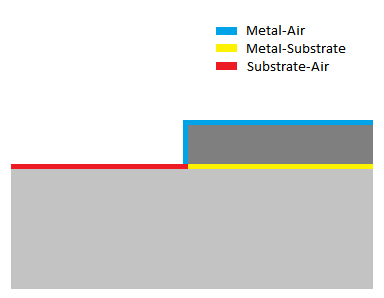
\includegraphics[scale=.8]{Figures/model}
		\caption{Simplification of the system including three lossy layers. The substrate and metal are depicted in light and dark grey respectively}
		\label{fig:model}
	\end{center}
\end{figure}



\section{Meshing}
To reduce simulation times the initial mesh is of critical importance. After each mesh refinement the fields are simulated anew. While CST is able to select regions of importance in the system where it should further refine the mesh, it can only do so after having simulated the fields. When establishing the initial mesh the importance of different regions of the system must be taken into account. Two \todo{two?} important steps taken to improve the initial mesh during this project are described below.   


\subsection{Ground}
To reduce the number of mesh elements, the ground pad is replaced by a sheet of PEC with zero thickness. Considering the field in the ground region is small compared to the field at the edges of the pads its contribution to the participation ratio is also small. Investing more computation time on the ground plane region by increasing the density of mesh elements there, would therefore also have limited impact on the participation ratio.
\subsection{Pads}
The pads being the source of the electric field, it is to be expected that the intensity will be greatest in this region. Furthermore, electric field lines tend to have a higher density at the edges of a metal \todo{Source or reference to Theory}. Considering this, the intensity of the electric field in the entire system is expected to be greatest around the edges of the metal pads. The initial mesh should reflect this by being very fine in these regions. In order to achieve this the edges of the metal pads are rounded as in figure \ref{fig:blending4}. A comparison between the resulting mesh and a standard initial mesh is depicted in figure \ref{fig:TotalMesh}. The difference is significant; an increase of mesh element count from 10776 to 590570. It would take CST around 8 iterations to achieve similar mesh element counts. The exact steps taken to achieve this in CST can be found in appendix \ref{appendix:CST_procedure}. 

\begin{figure}
	\centering
	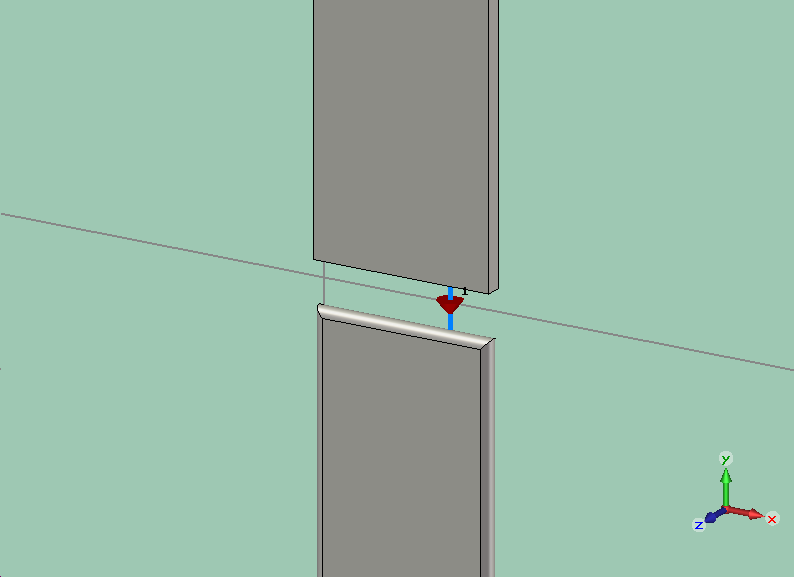
\includegraphics[scale=.5]{Figures/blending4}
	\caption{An illustration of the blending of the pad edges. The bottom pad has been blended whereas the top pad has not.}
	\label{fig:blending4}
\end{figure}

\begin{figure}
	\begin{tabular}{c c}
		\subfloat[Simple mesh] {{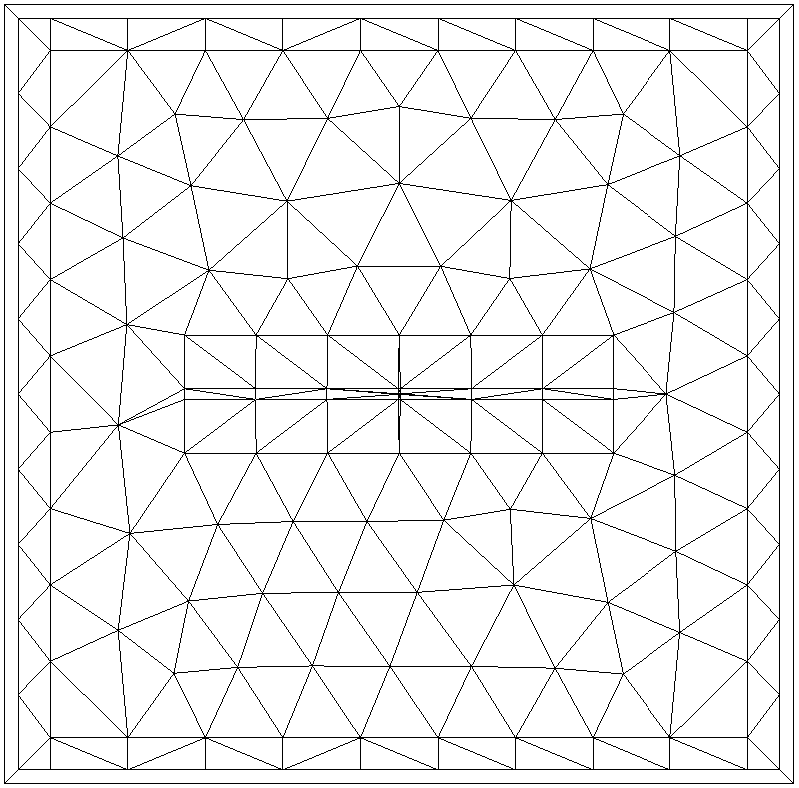
\includegraphics[width = \textwidth/2]{Figures/Anistropic_meshing/IBM_simple_cropped} }}
		& \subfloat[Refined mesh] {{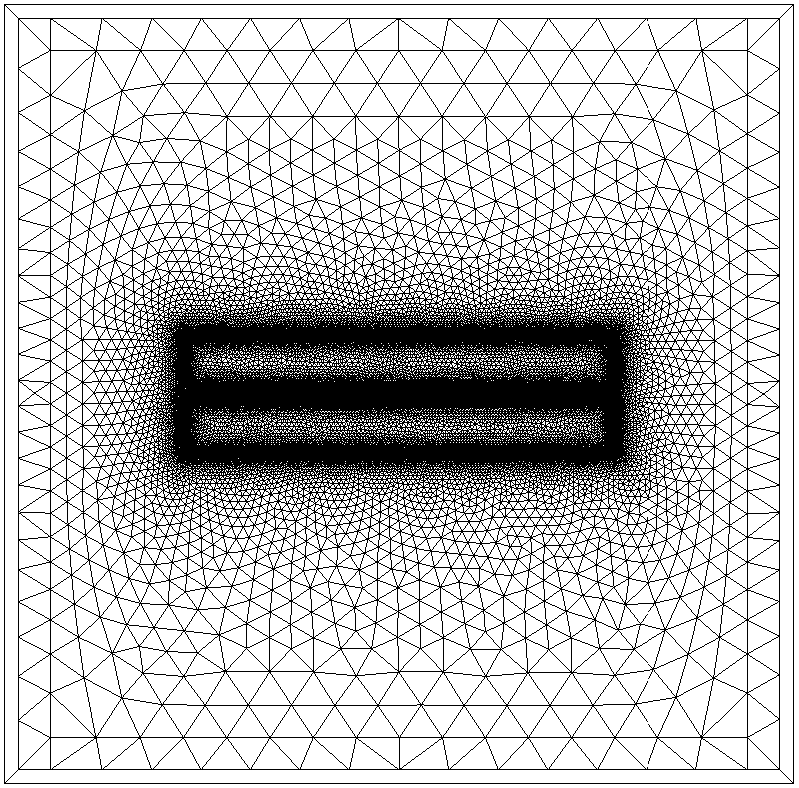
\includegraphics[width = \textwidth/2]{Figures/Anistropic_meshing/IBM_refined_cropped} }} \\
		\subfloat[Simple mesh, junction] {{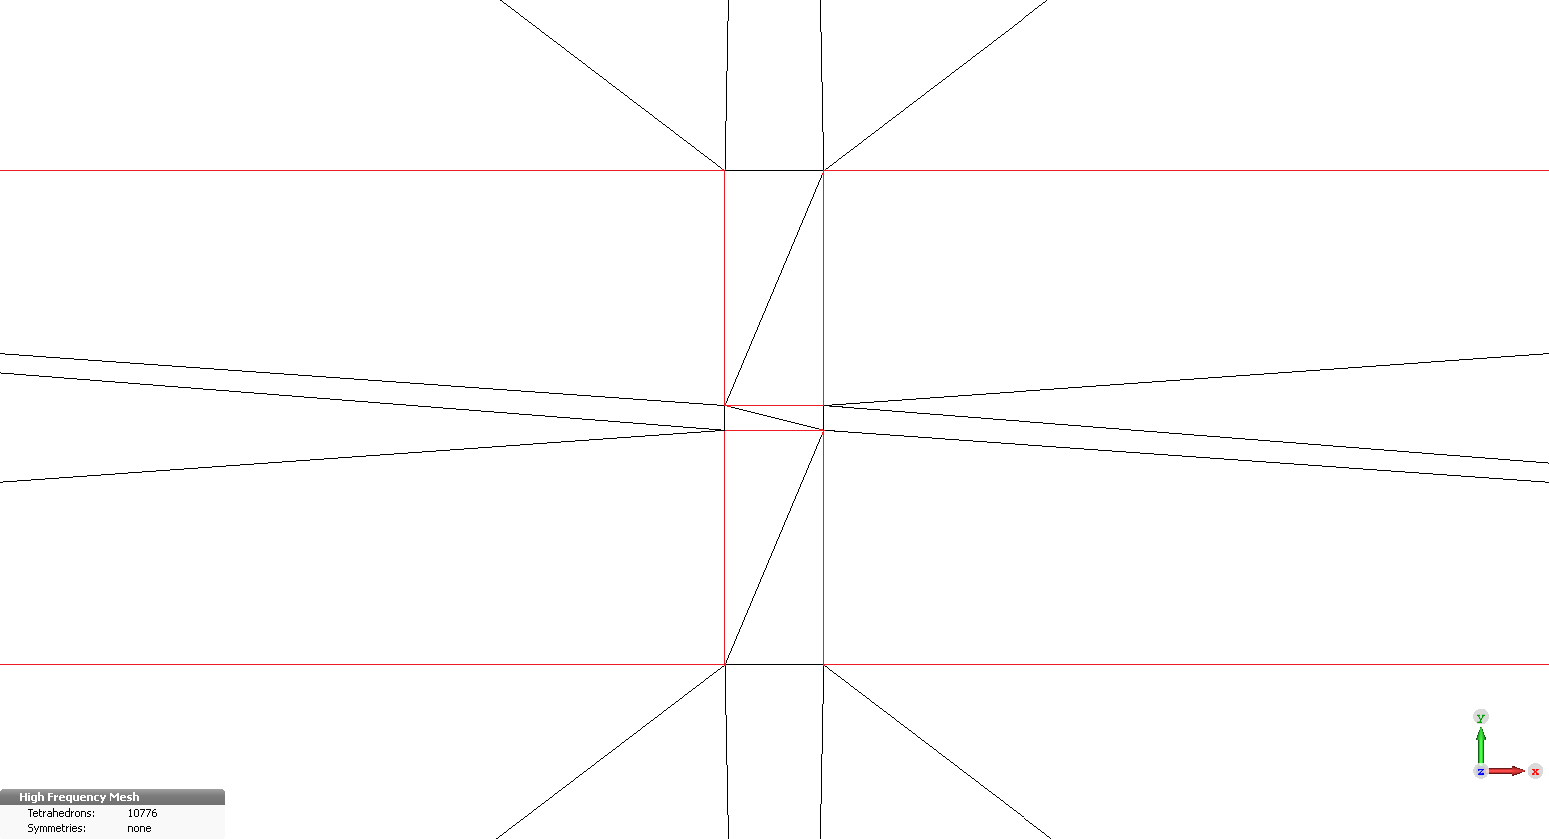
\includegraphics[width = \textwidth/2]{Figures/Anistropic_meshing/IBM_simple_zoomed_highlighted} }}
		& \subfloat[Refined mesh, junction] {{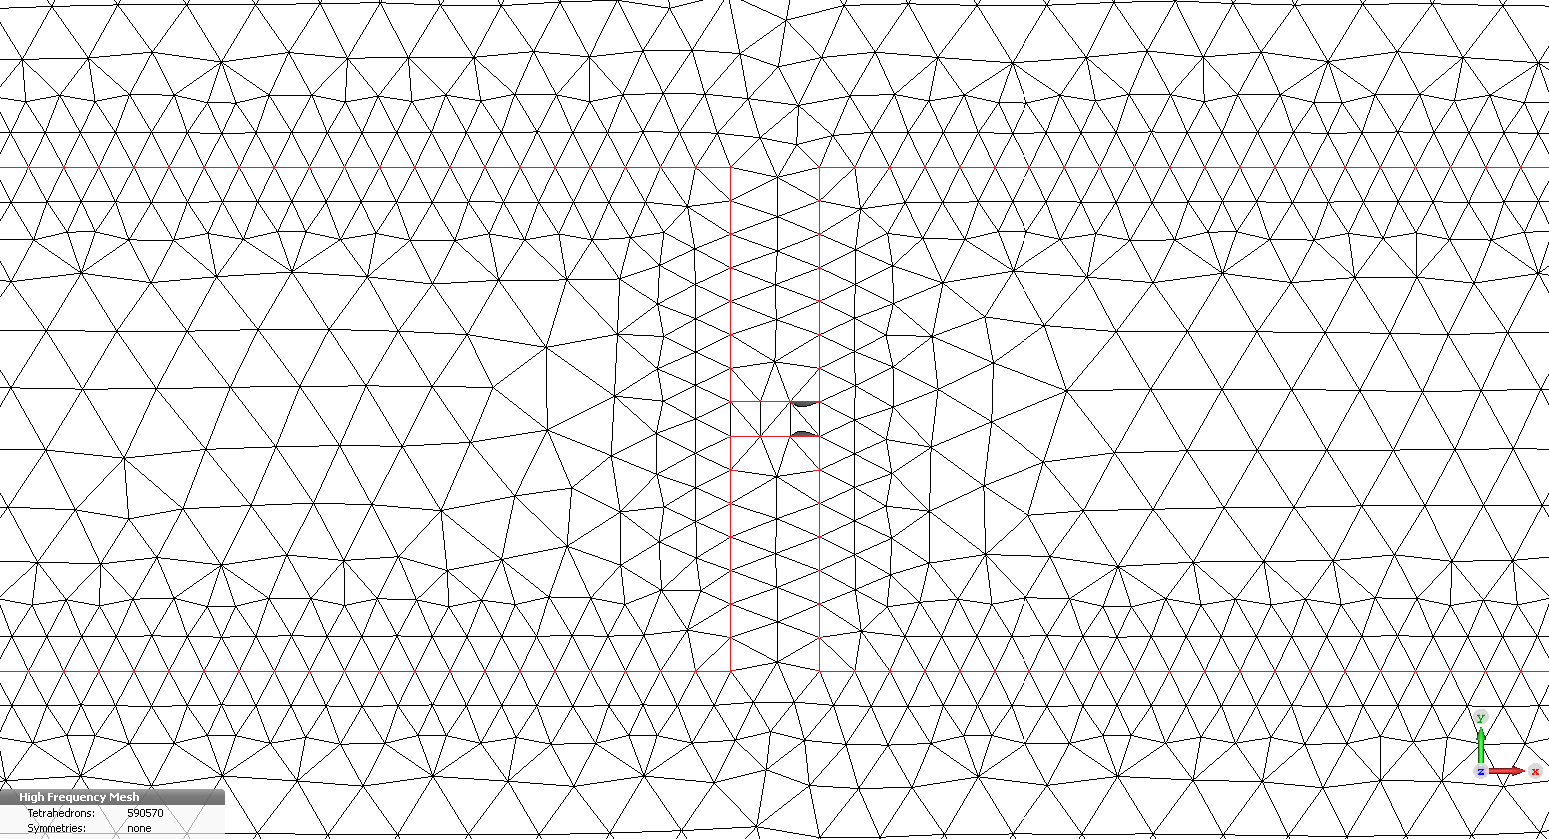
\includegraphics[width = \textwidth/2]{Figures/Anistropic_meshing/IBM_refined_zoomed_highlighted} }}
				
		
	\end{tabular}
	\caption{A comparison of the initial mesh before (a and c) and after (b and d) blending of the pad edges. (c) and (d) show the region close to the junction leads which are in the very centre in (a) and (b). The edges of the pads are highlighted in red. The total mesh element count is 10776 and 590570 for the simple and refined mesh respectively.}
	\label{fig:TotalMesh}
\end{figure}